\subsection{Менеджер состояний}
Для управления компонентами имитатора используется менеджер компонентов \texttt{ModbusIoManager}.
Установка компонентов производится с помощью экземпляра класса \texttt{ScenarioParser}, реализующего интерфейс \texttt{IParser}.
Этот интерфейс является общим для как для чтения файла сценария (\ref{lst:modbus_scenario_example_diagram}),
так и для файла тегов (листинг \ref{lst::modbus_tags_example}).
При чтении конфигурации проверяется, что каждый тег $t_i$ компонента,
управление над которым захватывается (\texttt{modbusio::ModbusData}) или условия выполнения переходов (\texttt{modbusio::ModbusDataRelationed}),
является элементов множества класса первичных данных, то есть $\forall t_i \in \mathbb{P}$ (см. раздел \ref{sec:ontology}).

На рисунке \ref{fig:modbus_class_components} показано отношение между менеджером \texttt{ModbusIoManager},
интерфейсом парсера \texttt{IParser} и интерфейсом \texttt{IModbusElementWriter}.
\begin{center}
    \begin{figure}[hb!]
        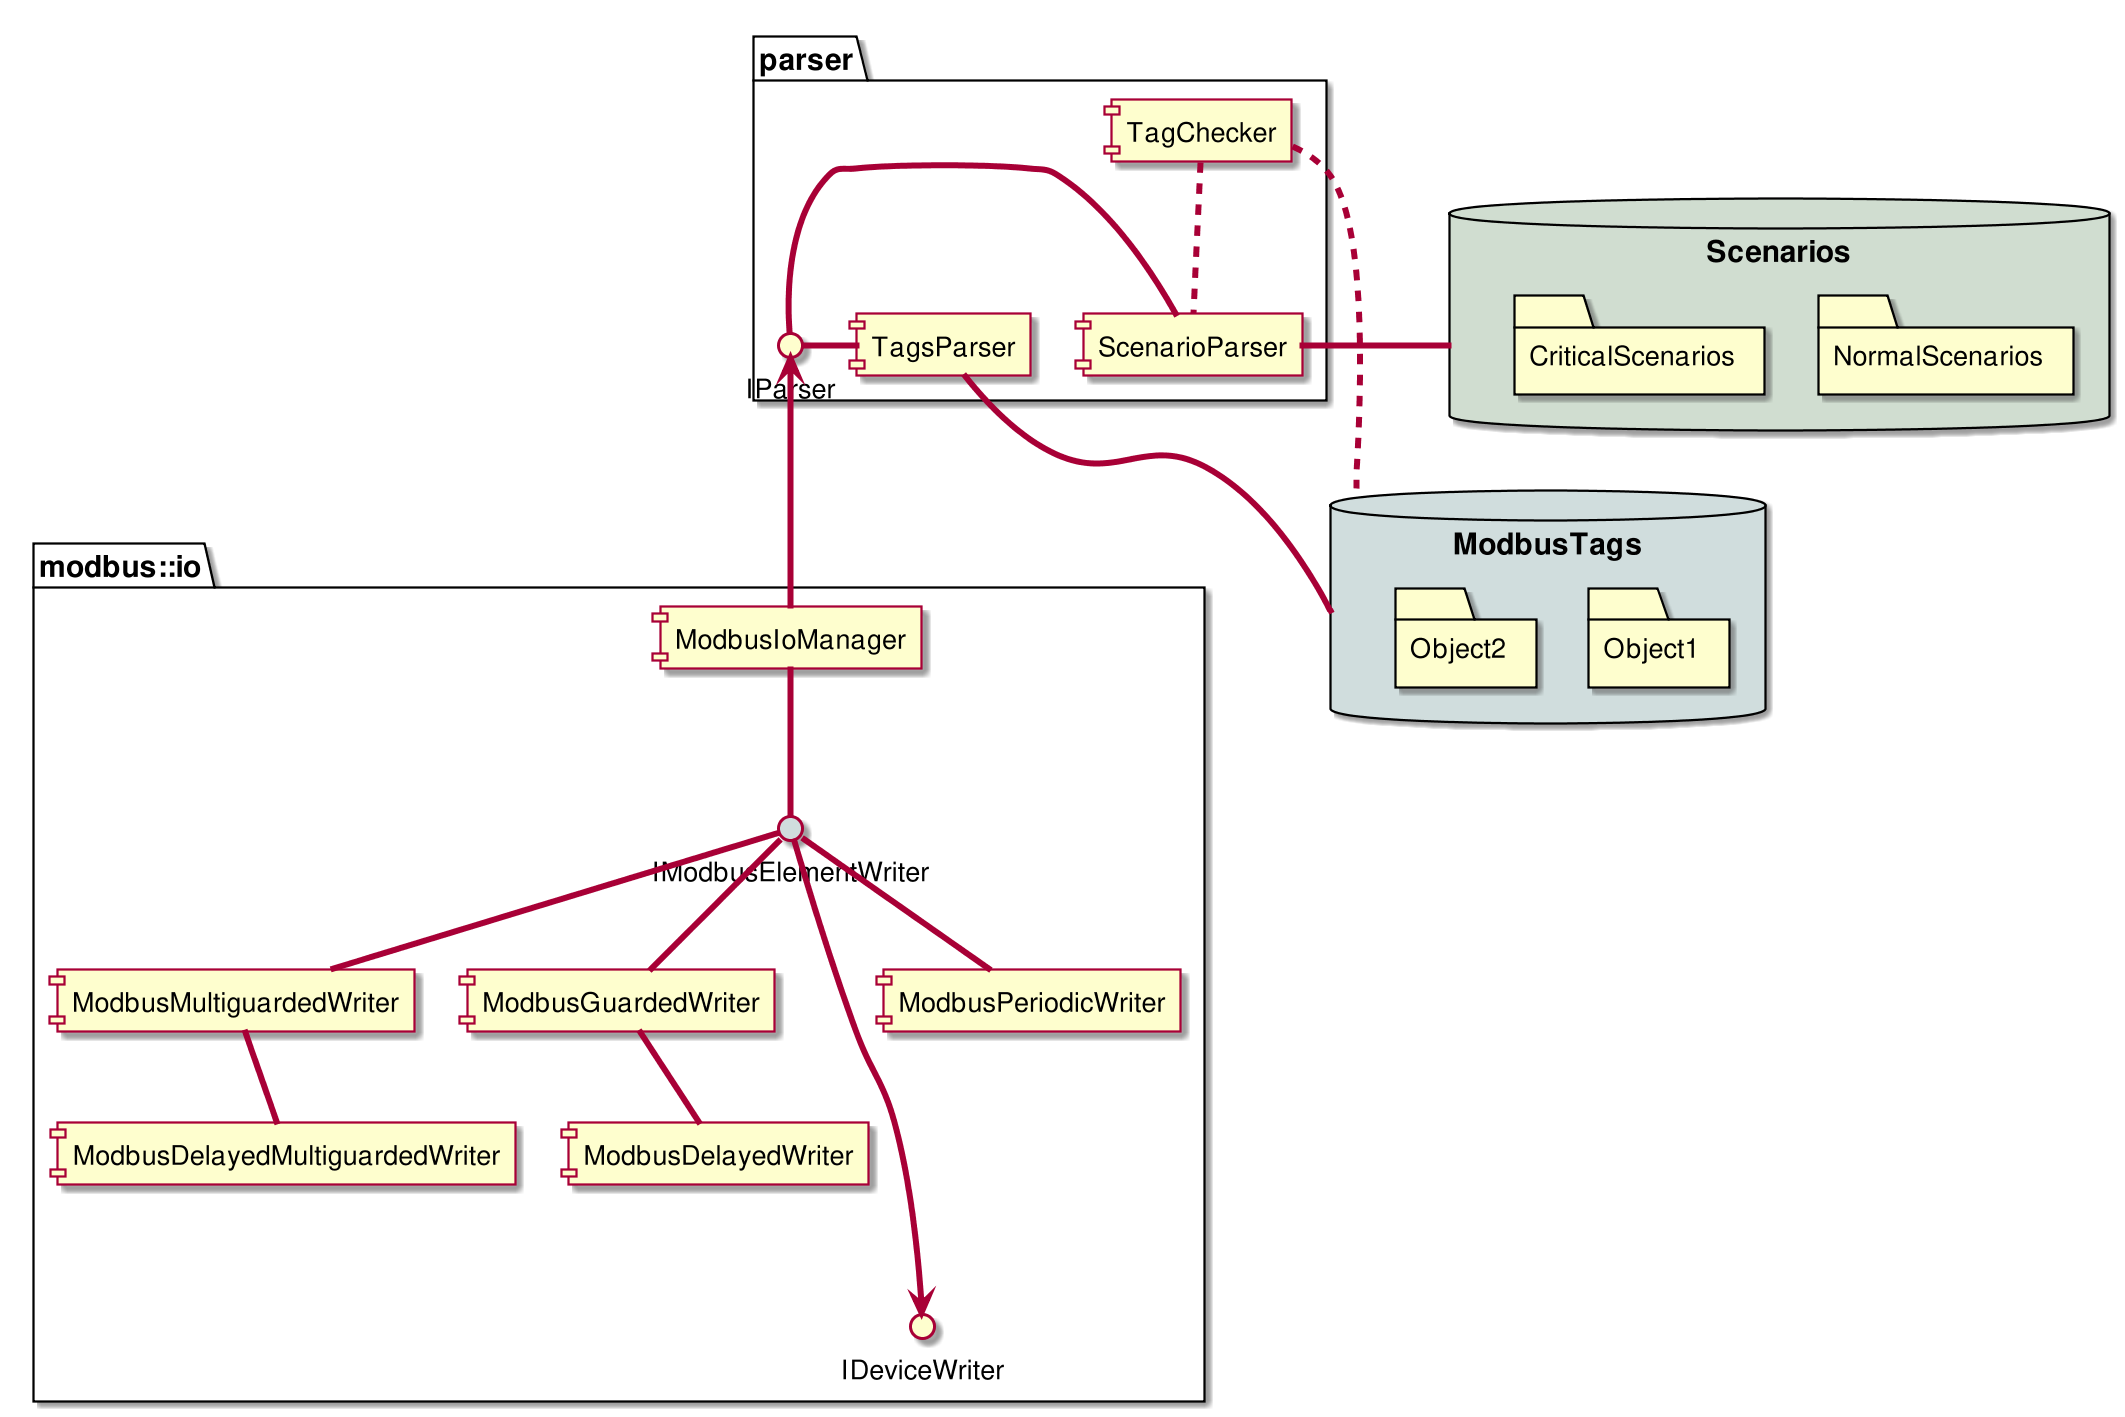
\includegraphics[width=.9\textwidth,keepaspectratio]{modbus_class_components}
        \caption{Композиция классов менеджера сценариев}\label{fig:modbus_class_components}
    \end{figure}
\end{center}

На рисунке \ref{fig:modbusiomanager_state_diagram} показаны активности менеджера.
\todo{Более информативный рисунок \ref{fig:modbuselementwriterimpl}.}
\begin{center}
    \begin{figure}
        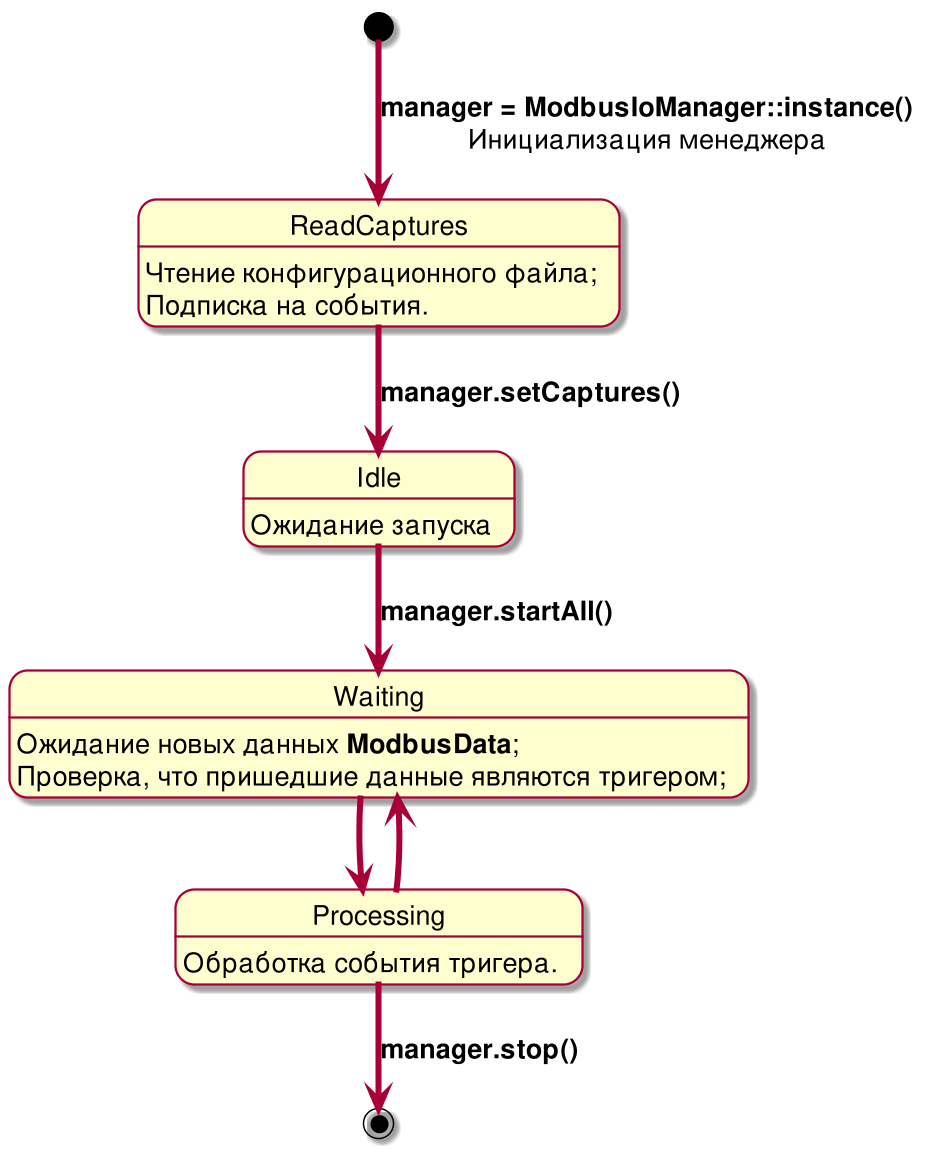
\includegraphics[width=.9\textwidth,keepaspectratio]{modbusiomanager_state_diagram}
        \caption{\todo{Жизненный цикл ModbusIoManager}}\label{fig:modbusiomanager_state_diagram}
    \end{figure}
\end{center}


Последовательность действий показана на рисунке \ref{fig:top_level_sequence} \cite[стр. 239]{book:oop:oop_analize}
\begin{center}
    \begin{figure}
        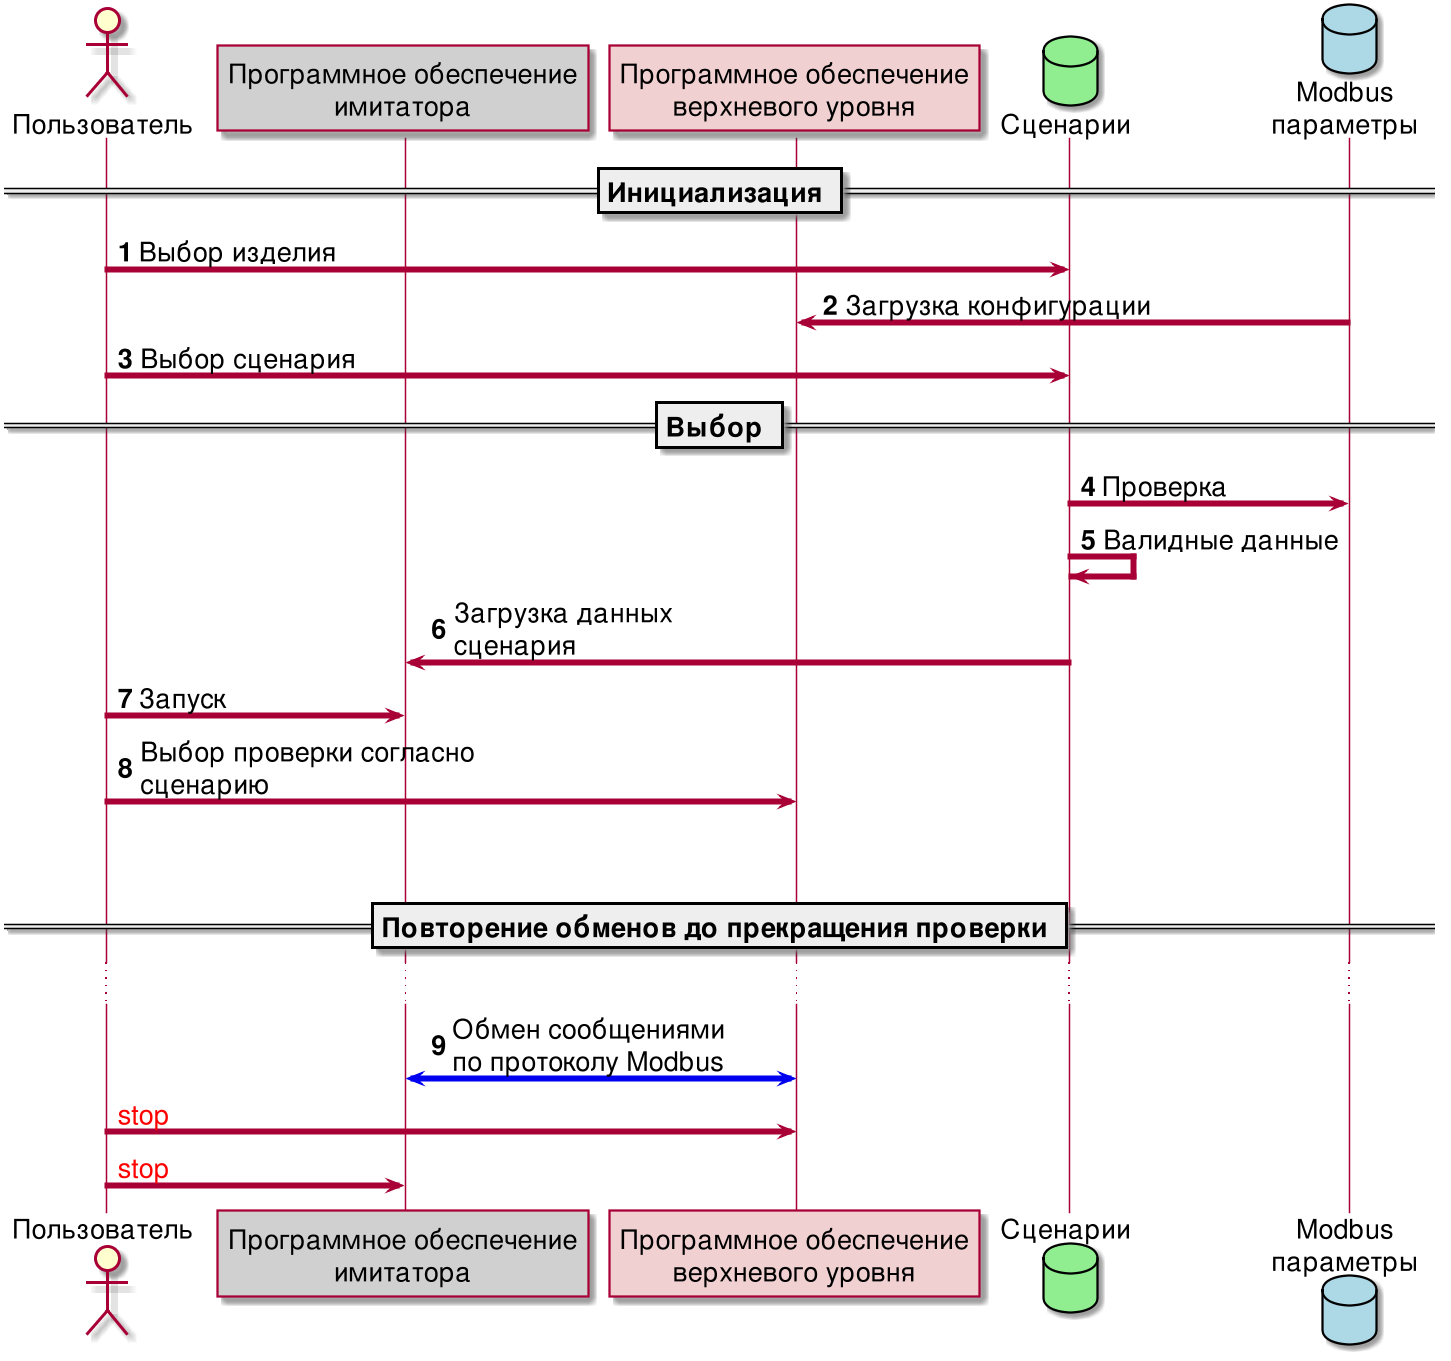
\includegraphics[width=.9\textwidth,keepaspectratio]{top_level.png}
        \caption{Последовательность действий при работе с имитатором}\label{fig:top_level_sequence}
    \end{figure}
\end{center}

\begin{center}
    \begin{figure}
        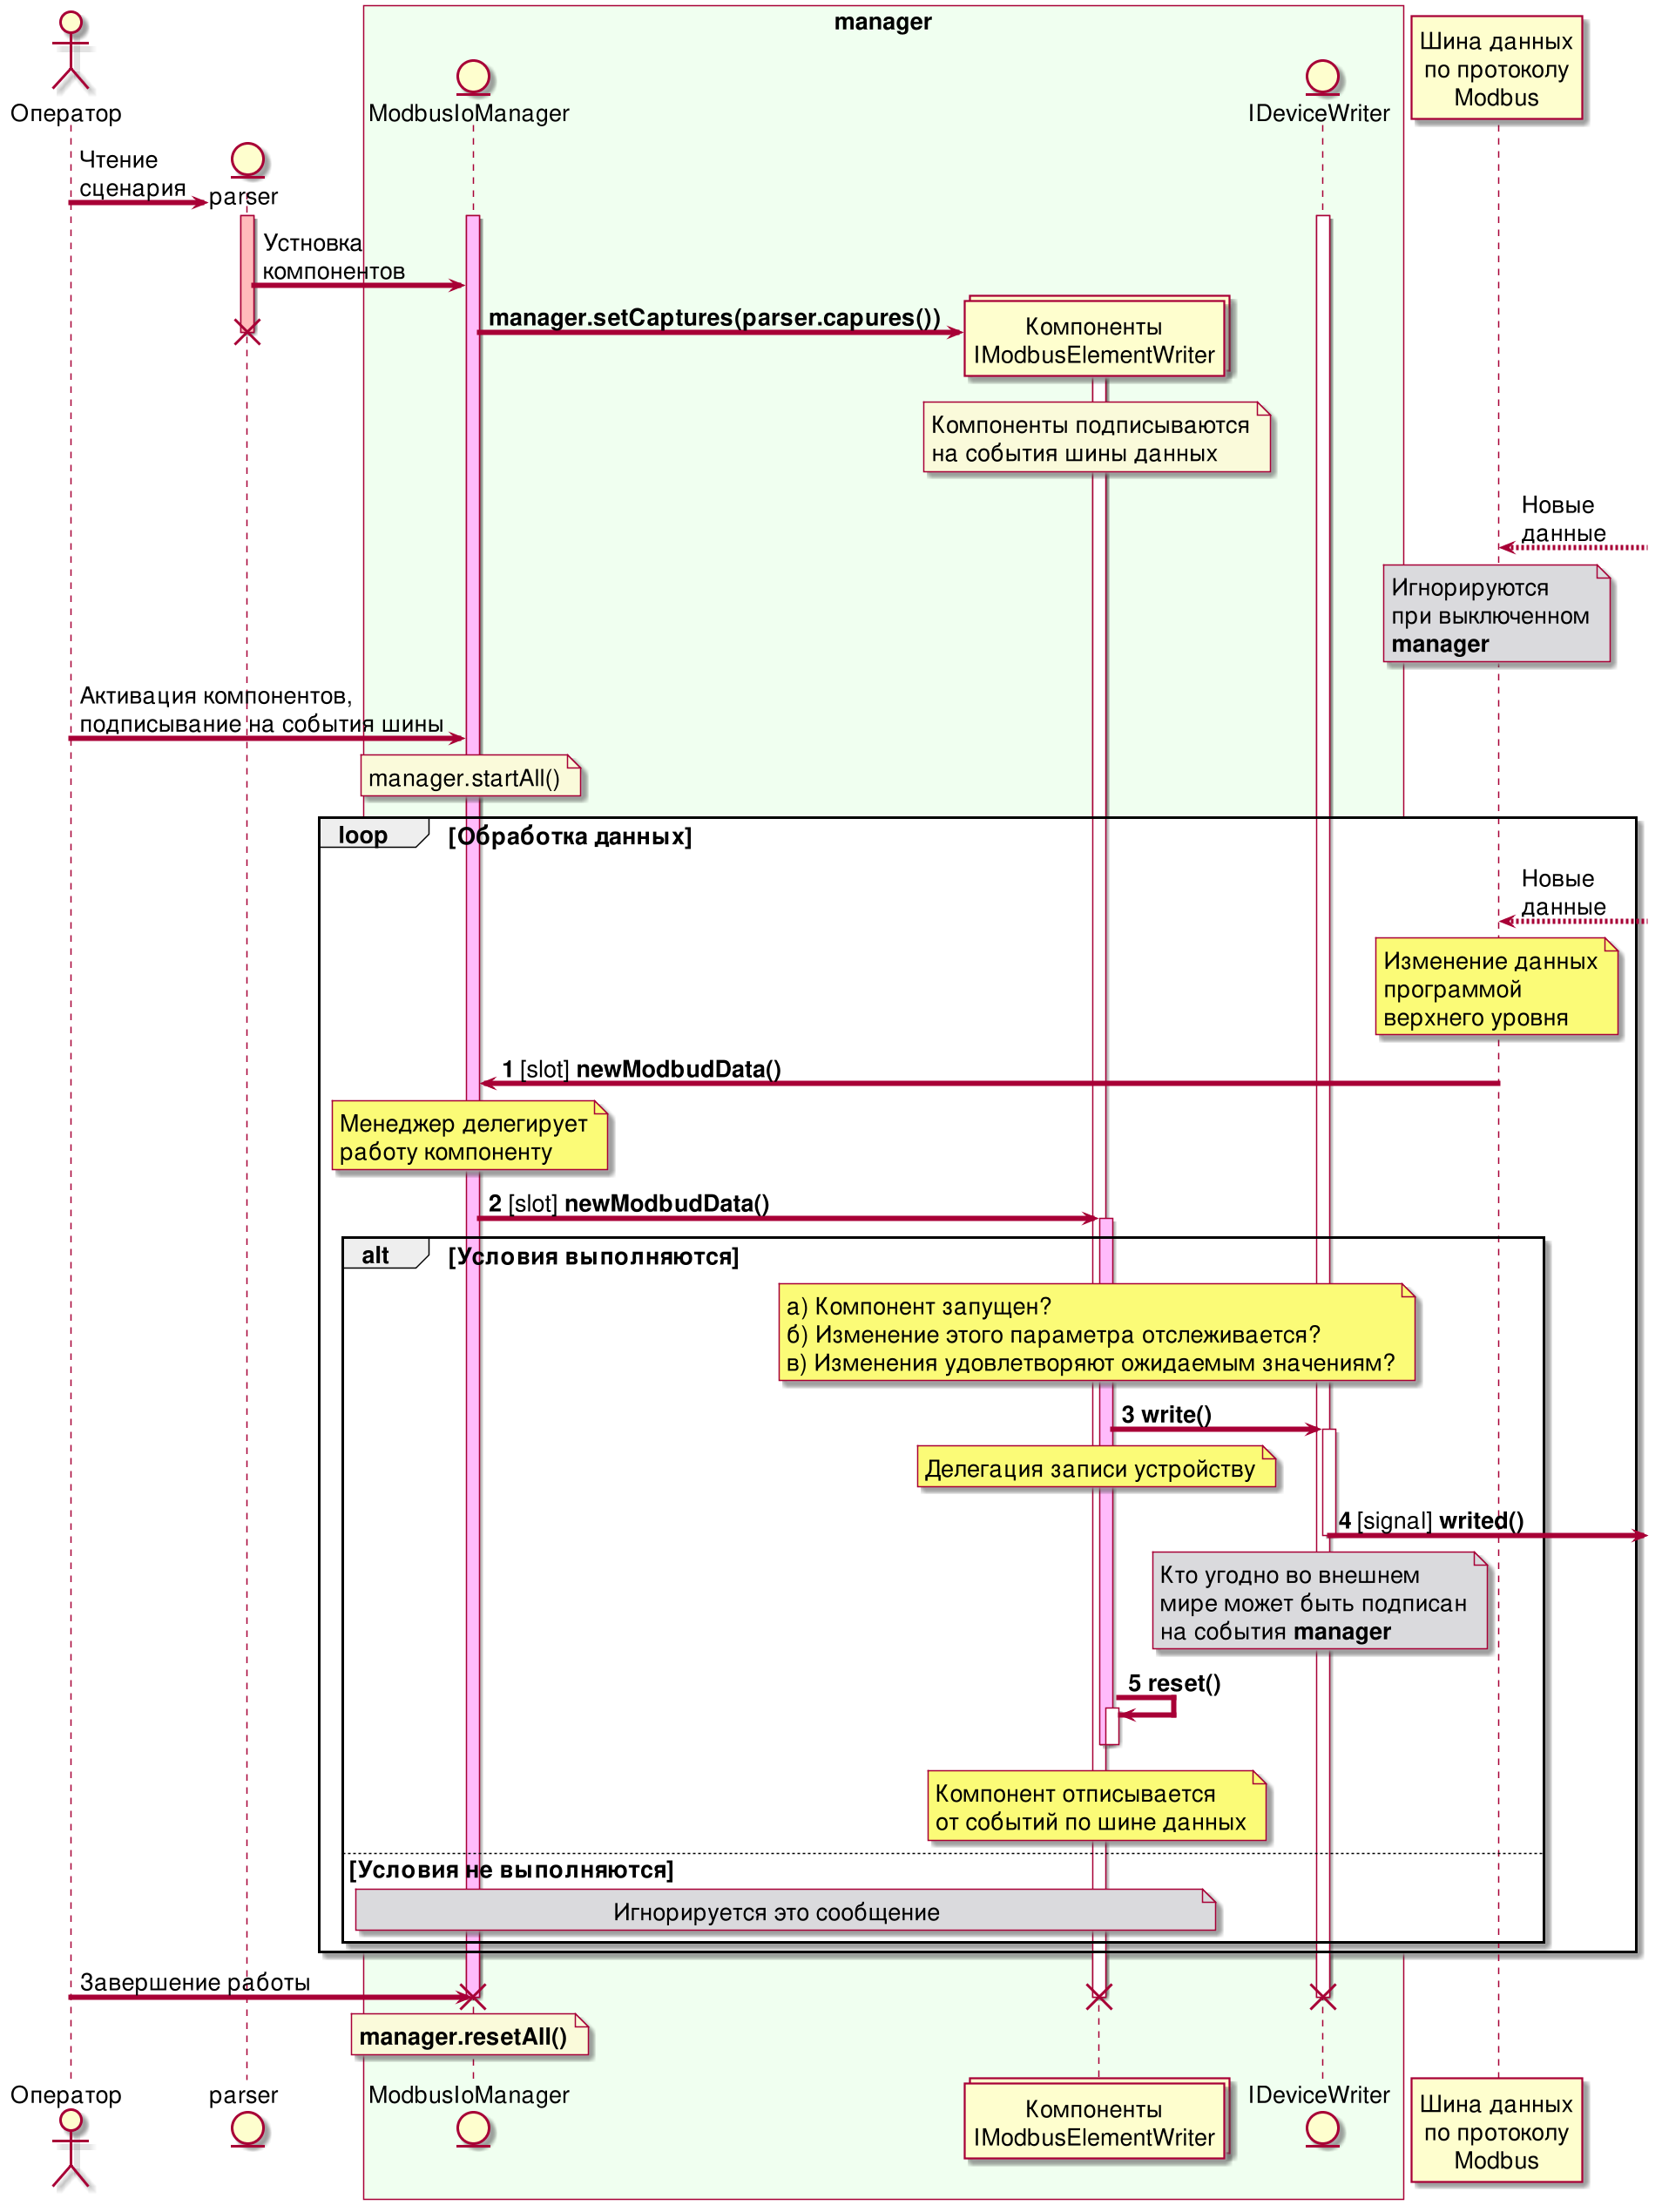
\includegraphics[width=.5\textwidth,keepaspectratio]{modbuselementwriterimpl.png}
        \caption{Взаимодействие компонентов с шиной данных (см. также листинг \ref{lst:tmpl_method_writerimpl})}\label{fig:modbuselementwriterimpl}
    \end{figure}
\end{center}


\clearpage
\section{Пример композиции для простейшего сценария}

Рассмотрим пример сценария на основе множества Modbus тегов из листинга \ref{lst:modbus_tags_example},
циклограмма которого представлена на рисунке \ref{fig:modbus_scenario_example_diagram},
сценарий приведен в листинге \ref{lst:modbus_scenario_example_diagram} в разделе приложения \ref{app:sec:modbus_scenario_example_diagram}.
Схема разметки приведена в листинге \ref{lst:modbus_tags_scenario_configs}.

\begin{landscape}
    \begin{center}
        \begin{figure}
            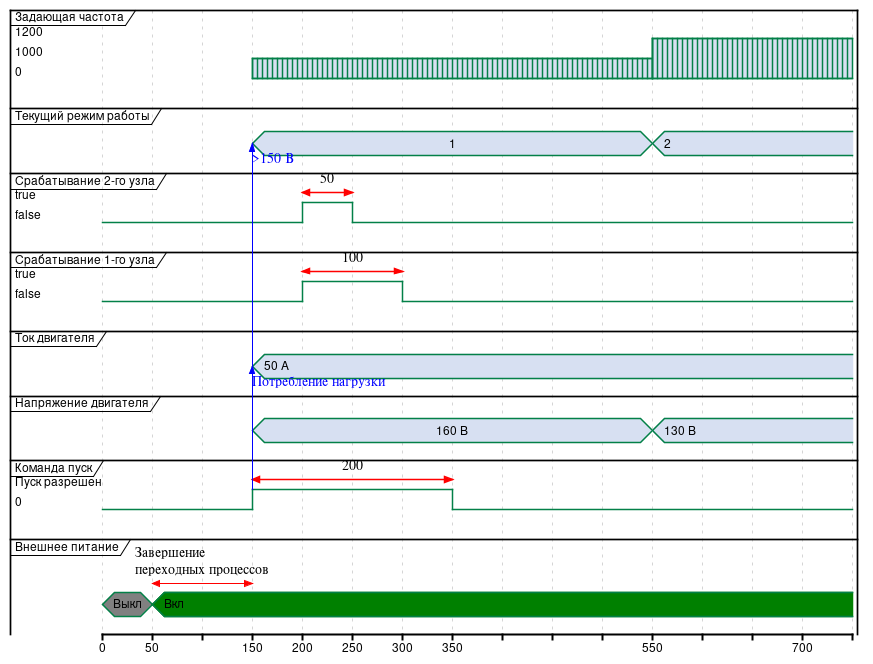
\includegraphics[height=.8\textheight,keepaspectratio]{modbus_scenario_example_diagram.png}
            \caption{Пример использования классов.}\label{fig:modbus_scenario_example_diagram}
        \end{figure}
    \end{center}
\end{landscape}
